\chapter{Discretización de dominios}
\graphicspath{{img/discret/}}

A continuación se presenta una visualización de las unidades geológicas obtenidas a partir de un estudio geológico realizado en Úmbita, Boyacá \cite{thesis:borda2017, geomodelr}. La representación de la geometría de estas unidades se hace a través del uso de mallas, el objeto de este capítulo.
\begin{figure}[H]
    \centering
    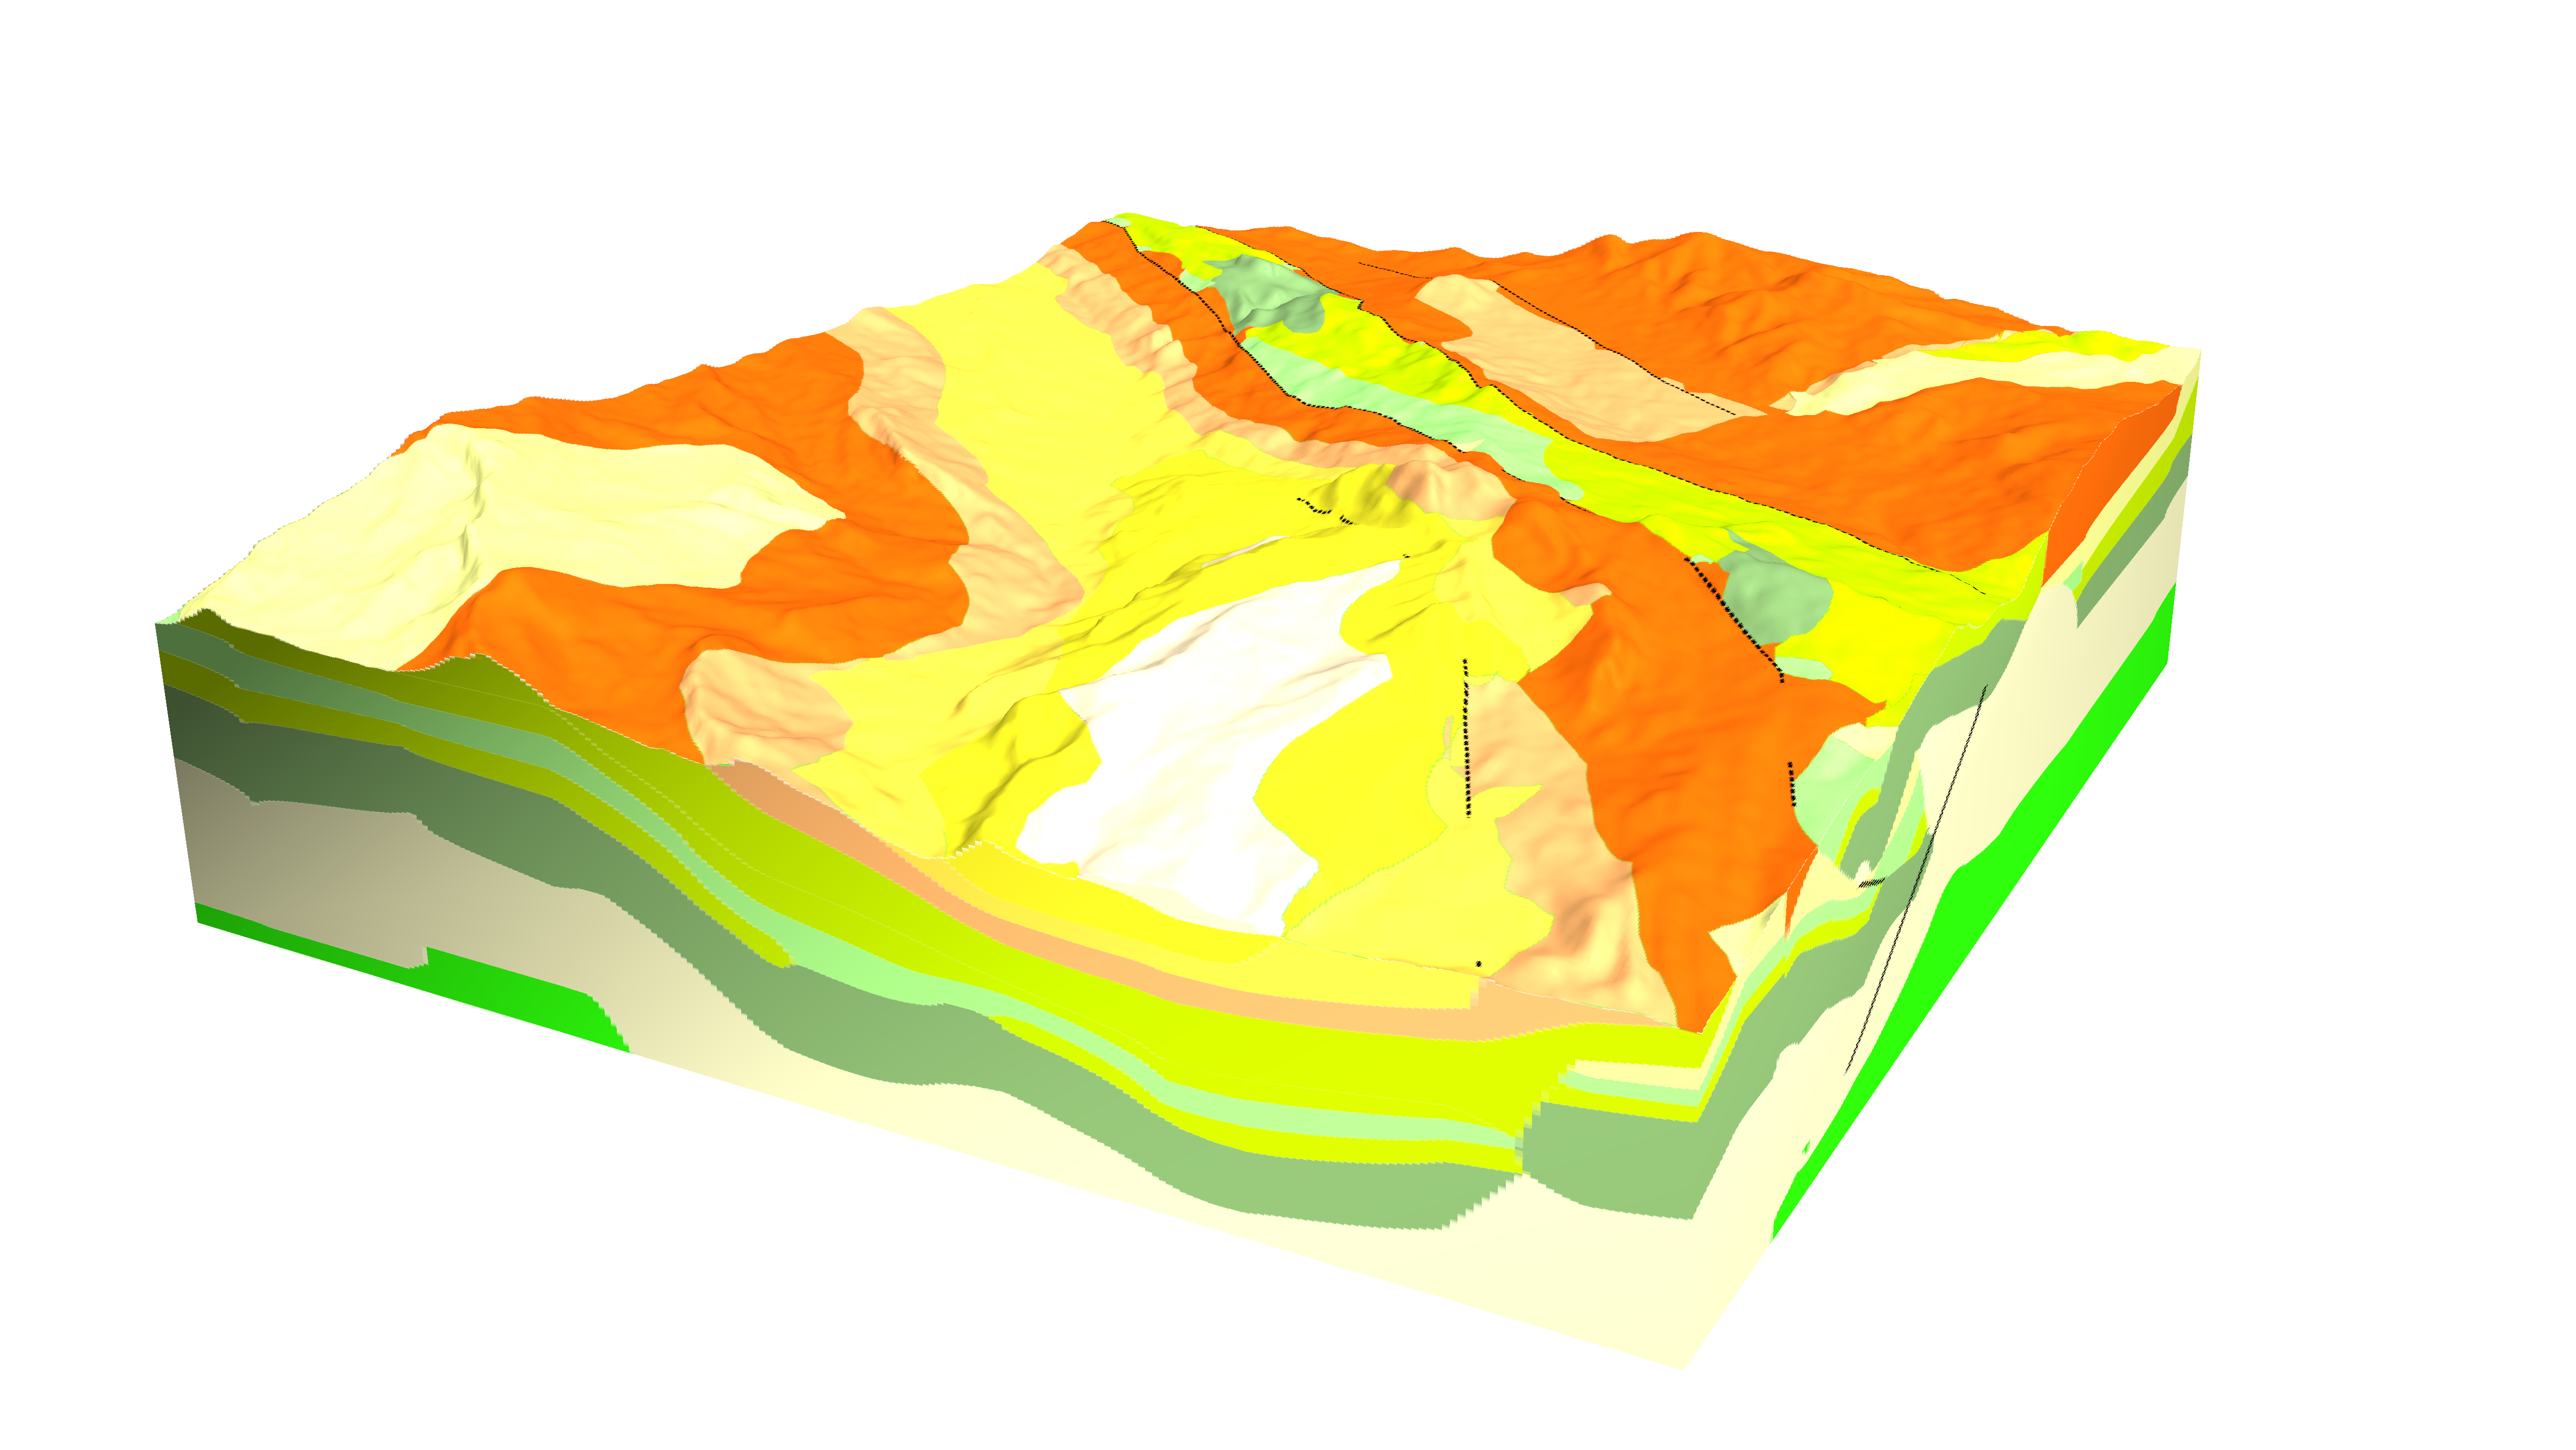
\includegraphics[width=12 cm]{Bloque.png}
    \caption{Visualización de las unidades geológicas obtenidas a partir del estudio presentado en \cite{thesis:borda2017}. Cortesía de \href{https://geomodelr.com/}{Geomodelr, Inc}.}
    \label{fig:geomodelr}
\end{figure}

Entre las unidades geológicas que se analizaron en este estudio se encuentra un (potencial) acuífero. Lograr describir la geometría del acuífero (u otras unidades geológicas) permitiría planear el desarrollo urbano alrededor. Por ejemplo, permitiría estimar el tamaño del mismo y asimismo la disponibilidad de agua potable en un futuro. La figura \ref{fig:unidades_aisladas} presenta dos de estas unidades geológicas.
\begin{figure}[H]
    \centering
    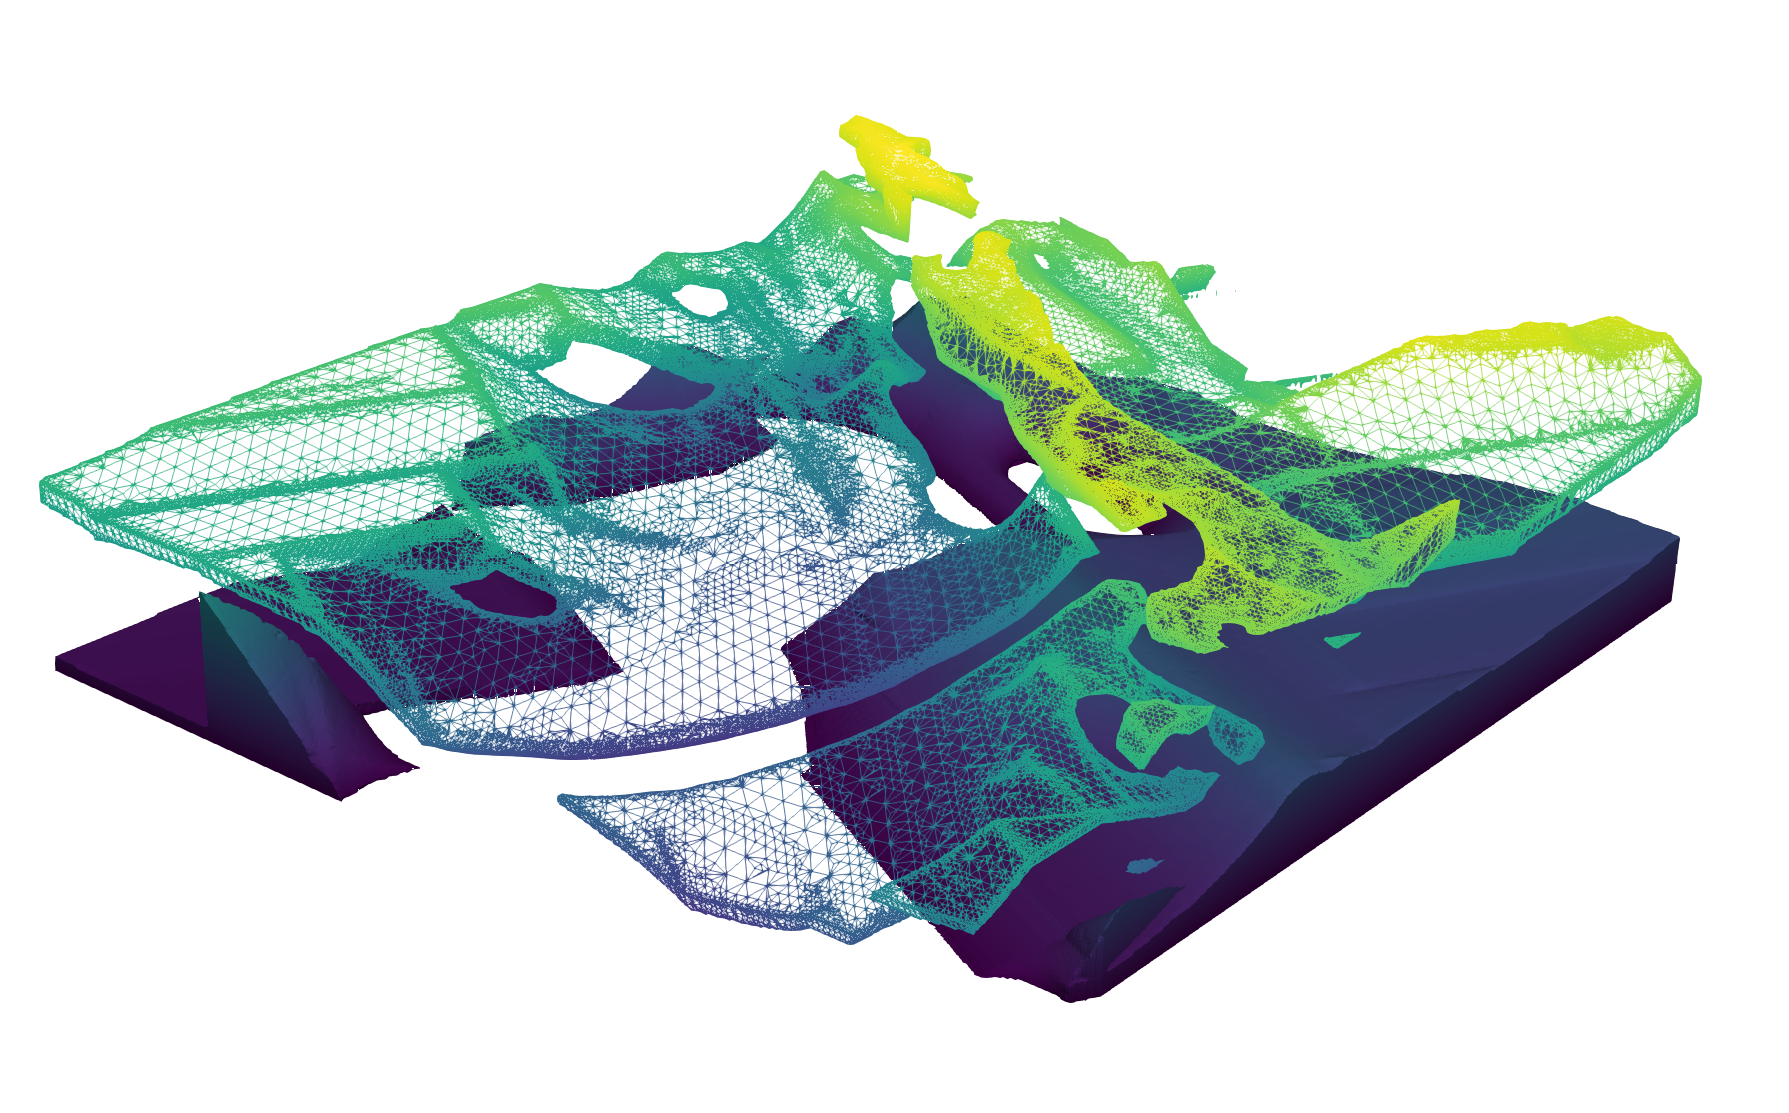
\includegraphics[width=12 cm]{bloques_malla.png}
    \caption{Visualización de dos las unidades geológicas obtenidas a partir 
    del estudio presentado en \cite{thesis:borda2017}. La unidad superior tiene 
    un volumen de 23 mil millones de m$^3$ y la inferior de 46 mil millones de 
    m$^3$. Datos cortesía de \href{https://geomodelr.com/}{Geomodelr, Inc}.}
    \label{fig:unidades_aisladas}
\end{figure}


\pagebreak
\section{Uso de mallas}

Las mallas se utilizan para representar geometrías en aplicaciones como:
\begin{itemize}
    \item \href{https://en.wikipedia.org/wiki/Computer_graphics}{Gráficos por computador}
    \begin{figure}[H]
        \centering
        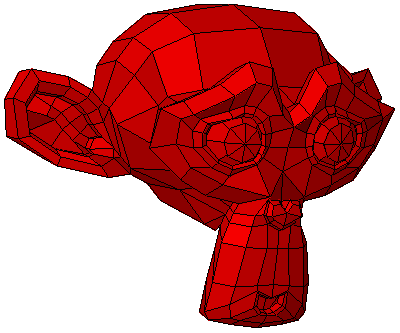
\includegraphics[width=5 cm]{Suzanne.pdf}\hspace{5mm}
        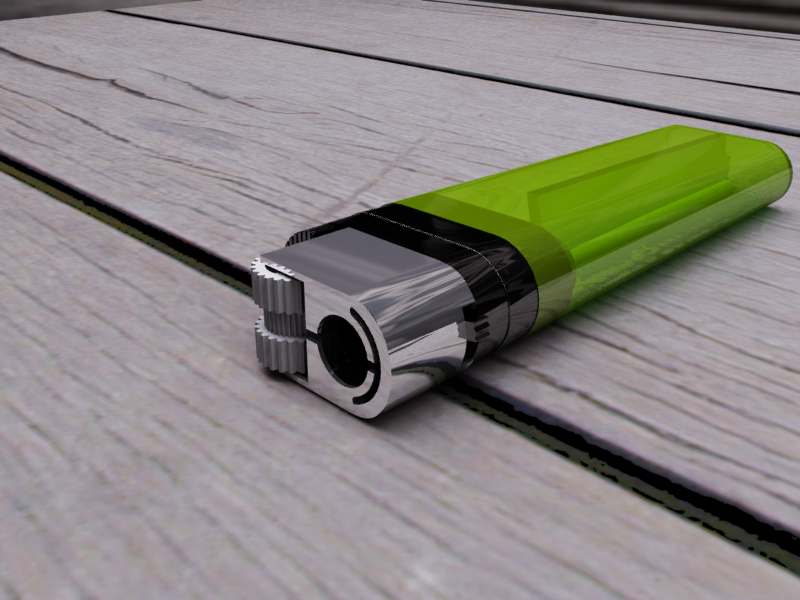
\includegraphics[width=5 cm]{Blender-yafray-render-lighter.png}
        \caption{Ejemplos de gráficos por computador. A la izquierda se tiene una malla que representa la cabeza de un mono. A la derecha se tiene un \href{https://en.wikipedia.org/wiki/Rendering_(computer_graphics)}{rénder} fotorrealista. Tomados de \cite{wiki:suzanne, wiki:encendedor}.}
    \end{figure}
    
    \item \href{https://en.wikipedia.org/wiki/Geographic_information_system}{Sistemas de información geográfica}
    \begin{figure}[H]
        \centering
        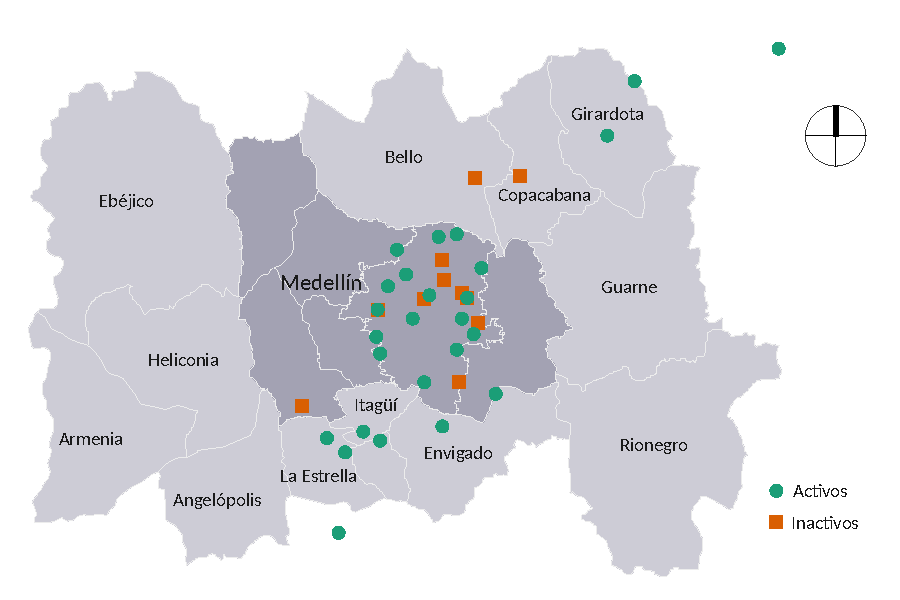
\includegraphics[width=9 cm]{red_acelerografica.pdf}
        \caption{Red acelerográfica de Medellín. Los círculos verdes representan estaciones activas. Mientras que los cuadrados naranja son estaciones inactivas. Datos de julio de 2017, tomados de SIATA\cite{SIATA_acelerografica}}
    \end{figure}
    
    \item \href{https://en.wikipedia.org/wiki/3D_printing}{Impresión 3D}
    \begin{figure}[H]
        \centering
        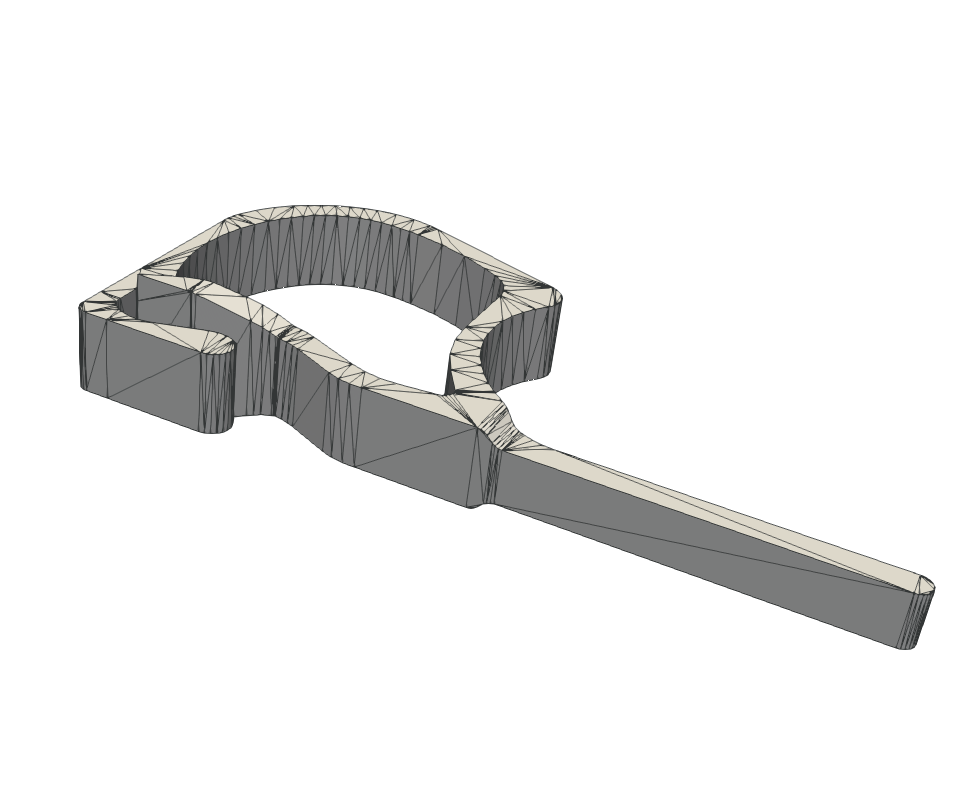
\includegraphics[width=5 cm]{soporte_vasos.png}\hspace{5mm}
        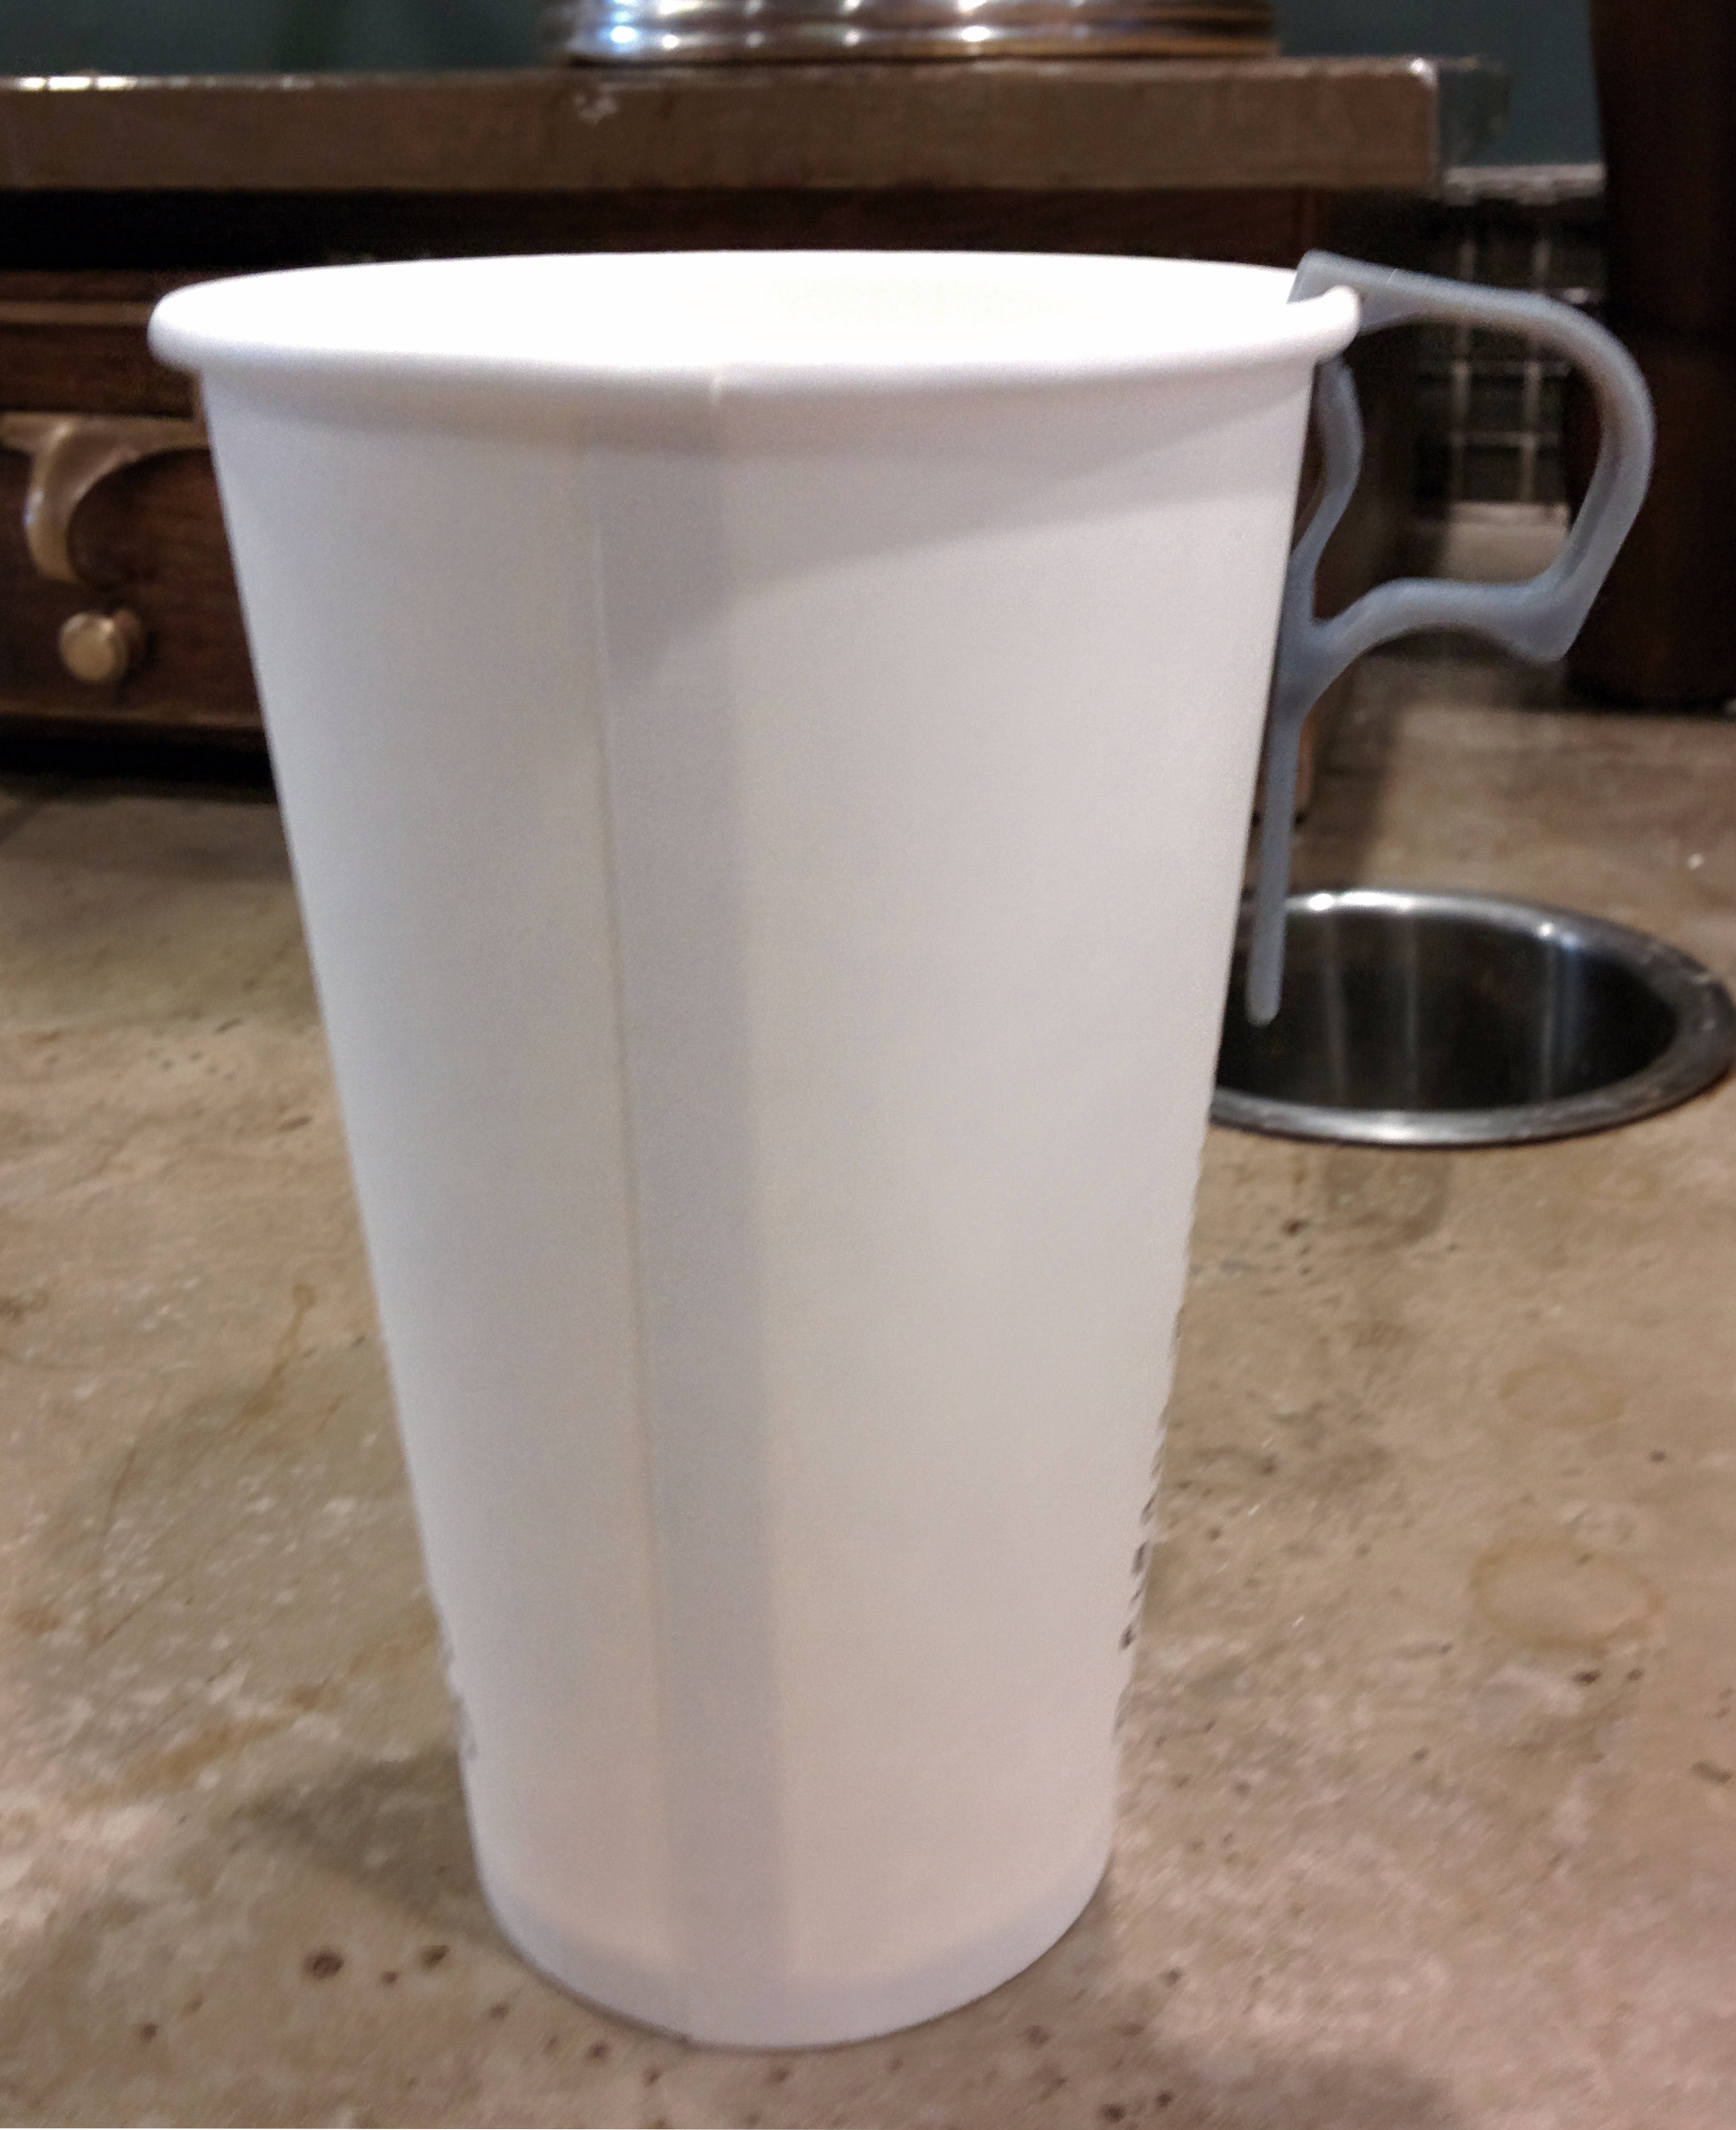
\includegraphics[width=4 cm]{cup_with_cup_holder.jpg}
        \caption{Ejemplo de impresión 3D: soporte para vasos de café. A la izquierda se tiene el modelo computacional de la pieza a imprimir. A la derecha se presenta la pieza impresa en un vaso de 12 onzas.}
    \end{figure}


    \item \href{https://en.wikipedia.org/wiki/Visualization_(graphics)}{Visualización}
    \begin{figure}[H]
        \centering
        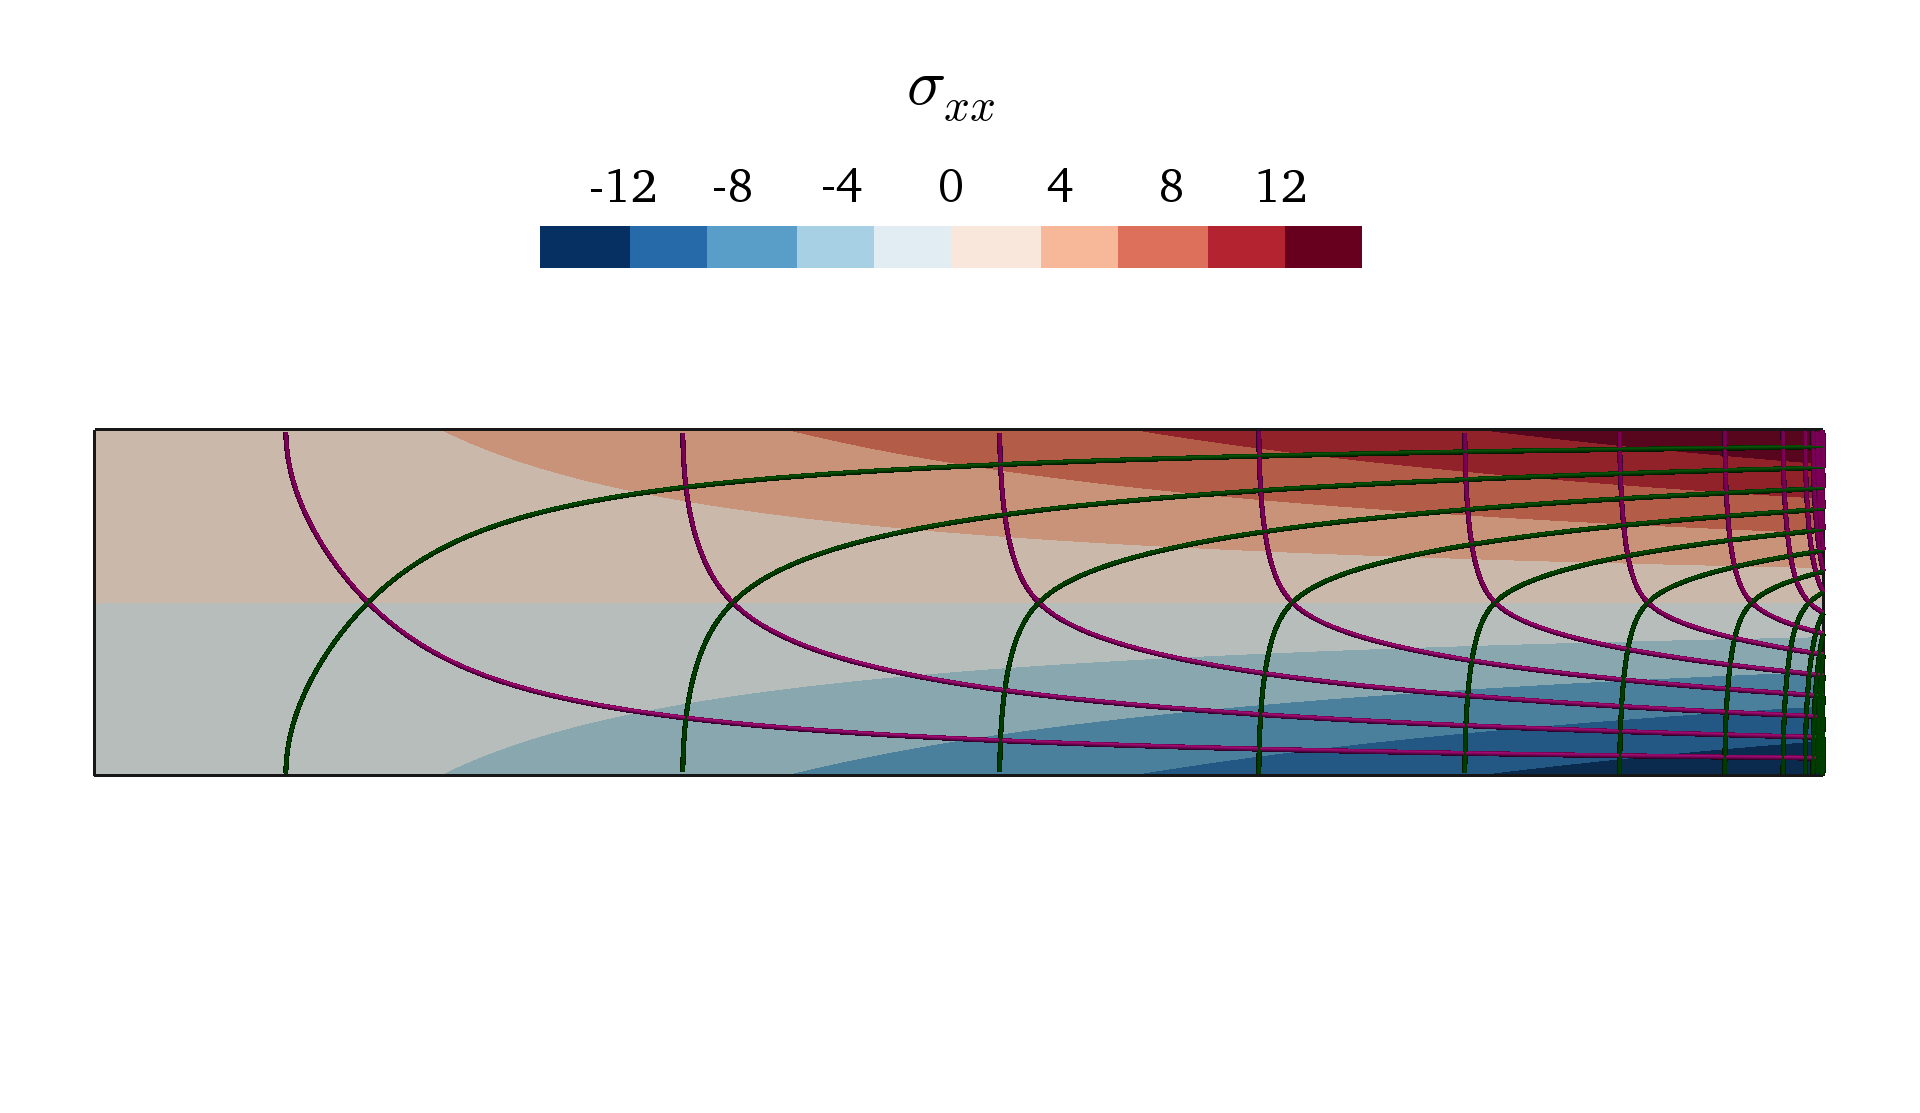
\includegraphics[width=12 cm]{viga_voladizo.png}
        \caption{Regiones de iso-esfuerzo para una viga en voladizo. Las líneas representan las direcciones principales del tensor.}
    \end{figure}

    \pagebreak
    \item Solución de ecuaciones diferenciales
    \begin{figure}[H]
        \centering
        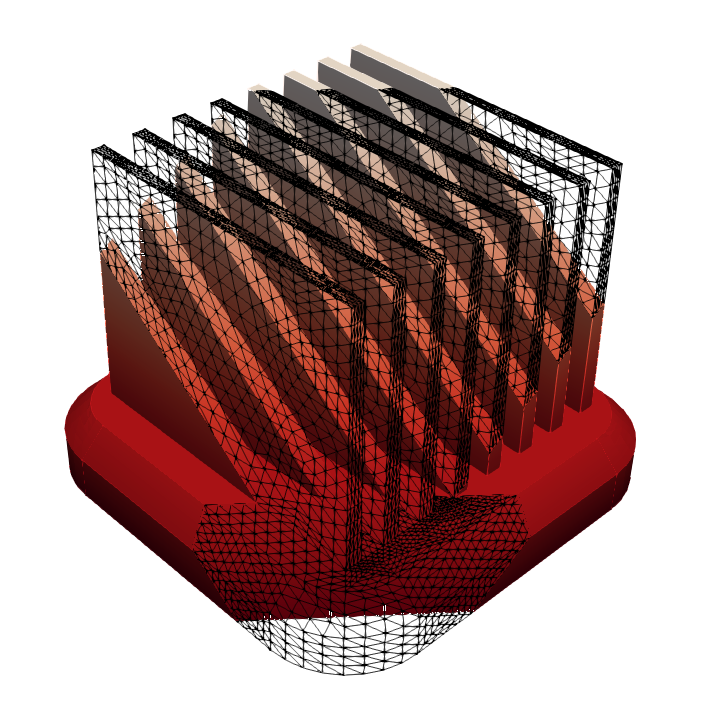
\includegraphics[width=10 cm]{disipador.png}
        \caption{Distribución de temperatura en un disipador de calor.}
    \end{figure}
\end{itemize}

\section{Concepto de malla}
Una malla es una colección de elementos cuya unión representa la forma de un dominio dado. Estos elementos suelen ser polígonos/poliedros simples como triángulos, tetraedros o hexaedros. Los elementos están organizados de tal forma que su intersección se da sólo en puntos, líneas o caras (en 3D).

Una malla puede estar conformada por elementos de diferente geometría. Una malla consta de un número finito de segmentos en una dimensión; segmentos, triángulos y cuadriláteros (quads) en dos dimensiones; y de los elementos anteriores, tetraedros (tets), pentaedros y hexaedros (hexes) en tres dimensiones.

\subsection{Mallas estructuradas}
Una malla es estructurada si la conectividad es la misma en todos los elementos interiores. Para mallas de cuadriláteros estos implica que en un vértice coinciden 4 elementos y para una de hexaedros coinciden 8. Los siguientes son ejemplos de mallas estructuradas.
\begin{figure}[H]
    \centering
    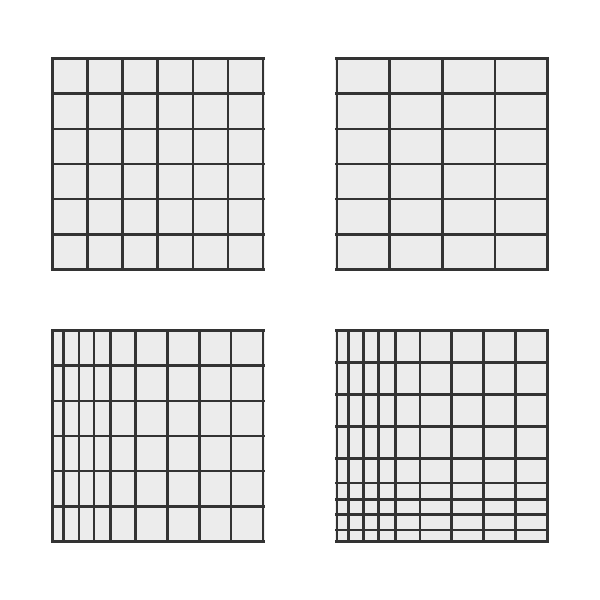
\includegraphics[width=4in]{mallas_estructuradas.pdf}
    \caption{Ejemplos de mallas estructuradas.}
\end{figure}


Debido a que la conectividad de la malla es la misma sólo es necesario almacenar la información de las coordenadas de los vértices. Una característica de las mallas estructuradas es que cada elemento puede indicarse por los índices $(i, j)$ en dos dimensiones, o $(i, j, k)$ en tres dimensiones, como se muestra a continuación.
\begin{figure}[H]
    \centering
    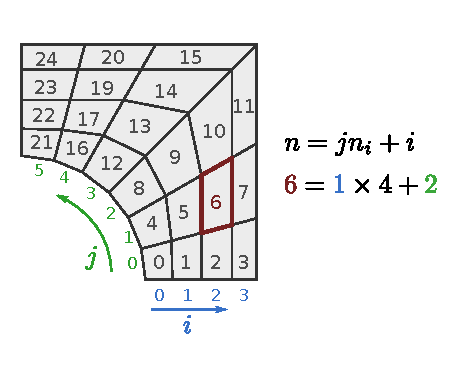
\includegraphics[width=8 cm]{malla_estruc_enumer.pdf}
    \caption{Ejemplo de enumeración de malla estructurada en dos dimensiones y su relación con dos índices $(i, j)$.}
\end{figure}


\subsection{Mallas no--estructuradas}
Una malla no--estructurada no tiene un patrón definido en la conectividad de los elementos. Este tipo de malla requiere almacenar las coordenadas de los vértices y las conectividades de todos los elementos.
\begin{figure}[H]
    \centering
    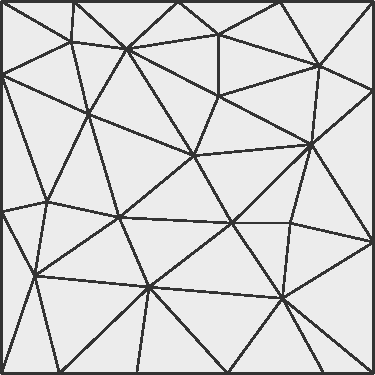
\includegraphics[width=2.3 in]{malla_no_estructurada.pdf}
    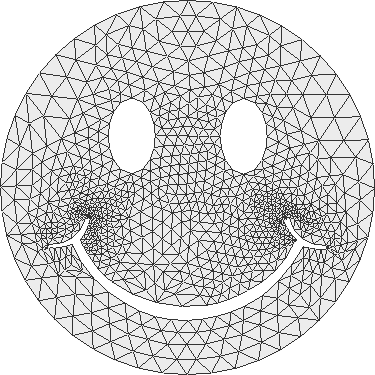
\includegraphics[width=2.5 in]{smiley_mesh.pdf}
    \caption{Ejemplos de mallas no--estructuradas.}
\end{figure}

Una ventaja de las mallas no--estructuradas sobre las mallas estructuradas es su versatilidad, ya que permiten representar geometrías más diversas más fácilmente.


\subsection{Representación de la malla}
La forma más común de representar una malla es usando la ubicación de sus nodos y la conectividad entre ellos para formar \emph{elementos}. Veamos un ejemplo para una malla simple dada en la siguiente figura.
\begin{figure}[H]
    \centering
    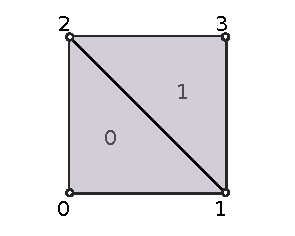
\includegraphics[width=2 in]{cuadrado_simple.pdf}
    \caption{Ejemplo de una malla simple formada por dos elementos triangulares y 4 nodos. La colección de elementos en este caso conforman un cuadrado.}
\end{figure}

Si asumimos que el nodo 0 tiene coordenadas (0, 0, 0) y el nodo 3 coordenadas (1, 1, 0) podemos definir la lista con las coordenadas de los nodos de la siguiente manera
\begin{minted}[mathescape,
numbersep=5pt,
gobble=0,
frame=lines,
framesep=2mm]{c}
0.0 0.0 0.0
1.0 0.0 0.0
0.0 1.0 0.0
1.0 1.0 0.0
\end{minted}
en donde vemos que la primera línea corresponde a las coordenadas del nodo 0 y así sucesivamente para los otros nodos. La lista con la conectividad de los elementos es la siguiente
\begin{minted}[mathescape,
numbersep=5pt,
gobble=0,
frame=lines,
framesep=2mm]{c}
0 1 2
1 3 2
\end{minted}
en donde podemos notar que el elemento 0 está conformado por los puntos (nodos) 0, 1 y 2 y el elemento 1 por los puntos 1, 3 y 2. En ambos casos la numeración de los nodos se hizo considerando una orientación antihoraria (con la mano derecha). La selección del primer nodo en el elemento es arbitraria, por ejemplo, el elemento 0 podría definirse como \texttt{(1 2 0)}, pero no como \texttt{(0 2 1)}, ya que este último está orientado en sentido horario.

\section{Creación de mallas}
Cuando tenemos geometrías sencillas podemos crear fácilmente mallas estructuradas para ellas, por ejemplo, usando Python. Sin embargo, el proceso se complica bastante cuando queremos crear mallas para geometrías arbitrarias o mallas no--estructuradas. Por esta razón se requiere de programas externos para la creación de mallas.

Veamos cómo visualizar un campo escalar dado por la función
\[f(x, y) = x^2 + y^3\]
en una sección de una elipse. Utilizando la función \texttt{meshgrid} de \texttt{numpy} podemos crear una rejilla definida por dos arreglos de números (coordenadas).

A continuación se presenta un bloque de código que permite generar la siguiente visualización.
\begin{figure}[H]
    \centering
    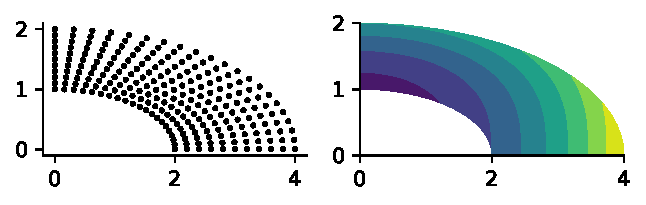
\includegraphics[width=5 in]{elipse_vis.pdf}
    \caption{Ejemplo de una malla estructura generada a partir de una parametrización de una sección de una elipse. No se muestra la conectividad, pero esta puede inferirse fácilmente.}
\end{figure}

\pagebreak
\begin{minted}[mathescape,
numbersep=5pt,
gobble=0,
frame=lines,
framesep=2mm]{python}
import numpy as np
import matplotlib.pyplot as plt

rad = np.linspace(1, 2, 11)
angle = np.linspace(0, np.pi/2, 21)
rad, angle = np.meshgrid(rad, angle)

a = 2.0 # semieje mayor
b = 1.0 # semieje menor
x = a * rad * np.cos(angle)
y = b * rad * np.sin(angle)
campo = x**2 + y**3

plt.figure(figsize=(5, 2.5))
plt.subplot(1, 2, 1)
plt.plot(x, y, color="black", marker=".", linewidth=0)
plt.axis("image")
plt.subplot(1, 2, 2)
plt.contourf(x, y, campo)
plt.axis("image")
plt.show()
\end{minted}

Para la creación de mallas en geometrías más complejas suelen utilizarse programas especializados. Algunos de estos son:
\begin{itemize}
    \item Gmsh
    \item Tetgen
    \item Triangle
    \item GiD
\end{itemize}

Nosotros nos centraremos en Gmsh\footnote{Gmsh es un software libre para la 
generación de mallas 2D y 3D para simulaciones de elementos finitos 
\cite{gmsh}.}.

La geometría en Gmsh se crea usando objetos geométricos que forman una jerarquía de la siguiente manera:
\begin{itemize}
\item \textbf{Puntos:} definidos por sus coordenadas.

\item \textbf{Líneas:} definidos por los puntos extremos en el caso de líneas rectas. Y definidos por el punto inicial, centro y punto final en el caso de arcos de circunferencia.

\item \textbf{Contornos (loops):} definidos por una unión de segmentos.

\item \textbf{Superficies:} definidas por un contorno.

\item \textbf{Volúmenes:} definidos por las superficies que forman la frontera.
\end{itemize}

La siguiente sección presenta estos conceptos con mayor detalle a través de un ejemplo.


\section{Ejemplo de creación de geometría y malla con Gmsh}
En este sección vamos a crear la geometría y malla para una sección transversal de un cilindro con un agujero coaxial. La geometría constará de dos superficies, cada una con un arco de \(\pi\) radianes. Este documento no pretende ser una introducción al manejo de Gmsh, para ello se sugiere el tutorial de la referencia \cite{avdis2012}, el tutorial oficial de Gmsh \cite{gmsh-tutorial} (para el manejo en modo texto) o los \emph{screencasts} oficiales \cite{gmsh-screencast} (para el manejo de la interfaz gráfica).

\subsection{Creación de la geometría}

\subsubsection{Puntos y líneas}
Llamemos \(r_\text{in}\) al radio interno y \(r_\text{ext}\) al radio externo. Estos parámetros podemos
incluirlos en el archivo de geometría con

\begin{minted}[mathescape,
numbersep=5pt,
gobble=0,
frame=lines,
framesep=2mm]{c}
// Parametros
rad_int = 2.0;  // Radio interior
rad_ext = 4.0;  // Redio exterior
\end{minted}


Los puntos base para la geometría estarían en las coordenadas
\begin{align*}
P1 &= (0.0, 0.0, 0.0)\\
P2 &= (-r_\text{ext}, 0.0, 0.0)\\
P3 &= ( r_\text{ext}, 0.0, 0.0)\\
P4 &= (-r_\text{int}, 0.0, 0.0)\\
P5 &= (r_\text{int}, 0.0, 0.0)\, .
\end{align*}

Que en el archivo de entrada serían

\begin{minted}[mathescape,
numbersep=5pt,
gobble=0,
frame=lines,
framesep=2mm]{c}
// Puntos
Point(1) = {0.0, 0.0, 0, 1.0};
Point(2) = {-rad_ext, 0.0, 0, 1.0};
Point(3) = { rad_ext, 0.0, 0, 1.0};
Point(4) = {-rad_int, 0.0, 0, 1.0};
Point(5) = { rad_int, 0.0, 0, 1.0};
\end{minted}


Los arcos de circunferencia se definen mediante la terna (Punto inicial, Centro, Punto final). El arco subtendido debe ser menor o igual a \(\pi\) radianes.

Los puntos y líneas pueden verse en la siguiente figura
\begin{figure}[H]
    \centering
    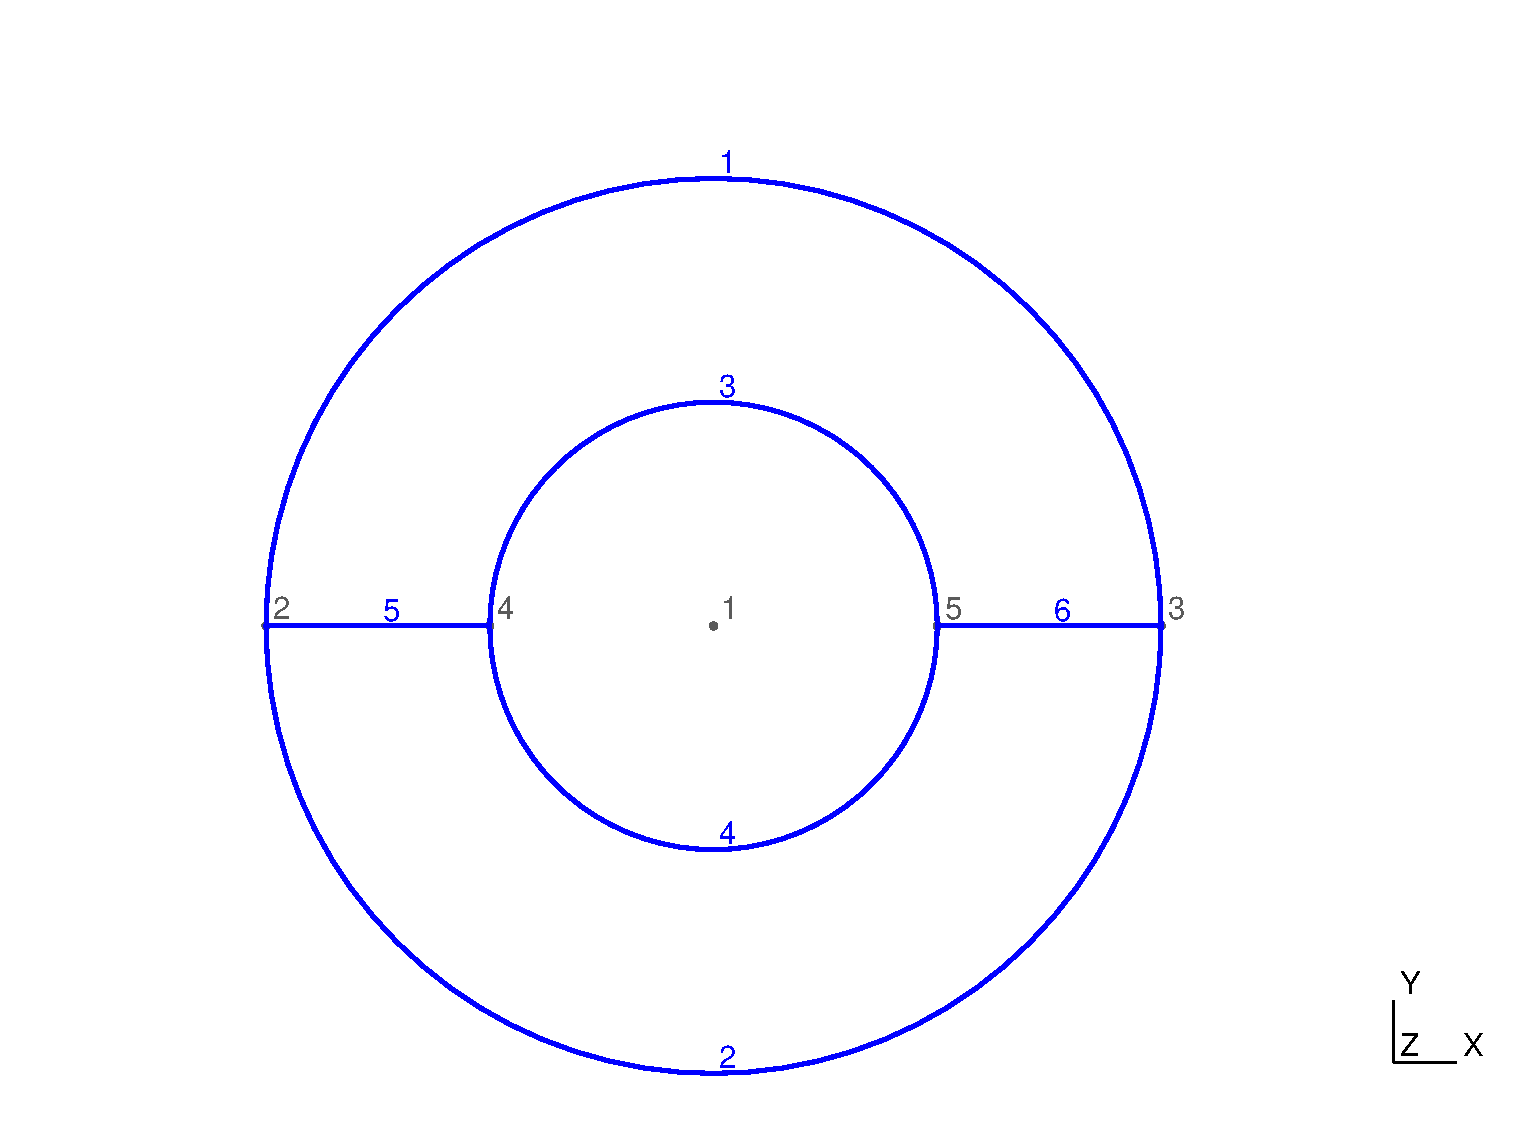
\includegraphics[width=12 cm]{anillo.pdf}
    \caption{Líneas y puntos para la geometría. Los puntos se representan en gris y las líneas en azul}
    \label{fig:geo_puntos}
\end{figure}

La definición de las líneas sería la siguiente
\begin{minted}[mathescape,
numbersep=5pt,
gobble=0,
frame=lines,
framesep=2mm]{c}
// Lineas
Circle(1) = {3, 1, 2};
Circle(2) = {2, 1, 3};
Circle(3) = {5, 1, 4};
Circle(4) = {4, 1, 5};
Line(5) = {2, 4};
Line(6) = {5, 3};
\end{minted}

\subsubsection{Contornos y superficies}
Los contornos son conjuntos de líneas que forman una figura cerrada. Por convención, elegimos el
sentido antihorario como el sentido positivo. En este caso, los contornos o bucles\footnote{En inglés se denominan \emph{loops}.} se definen como muestra la siguiente figura.
\begin{figure}[h]
    \centering
    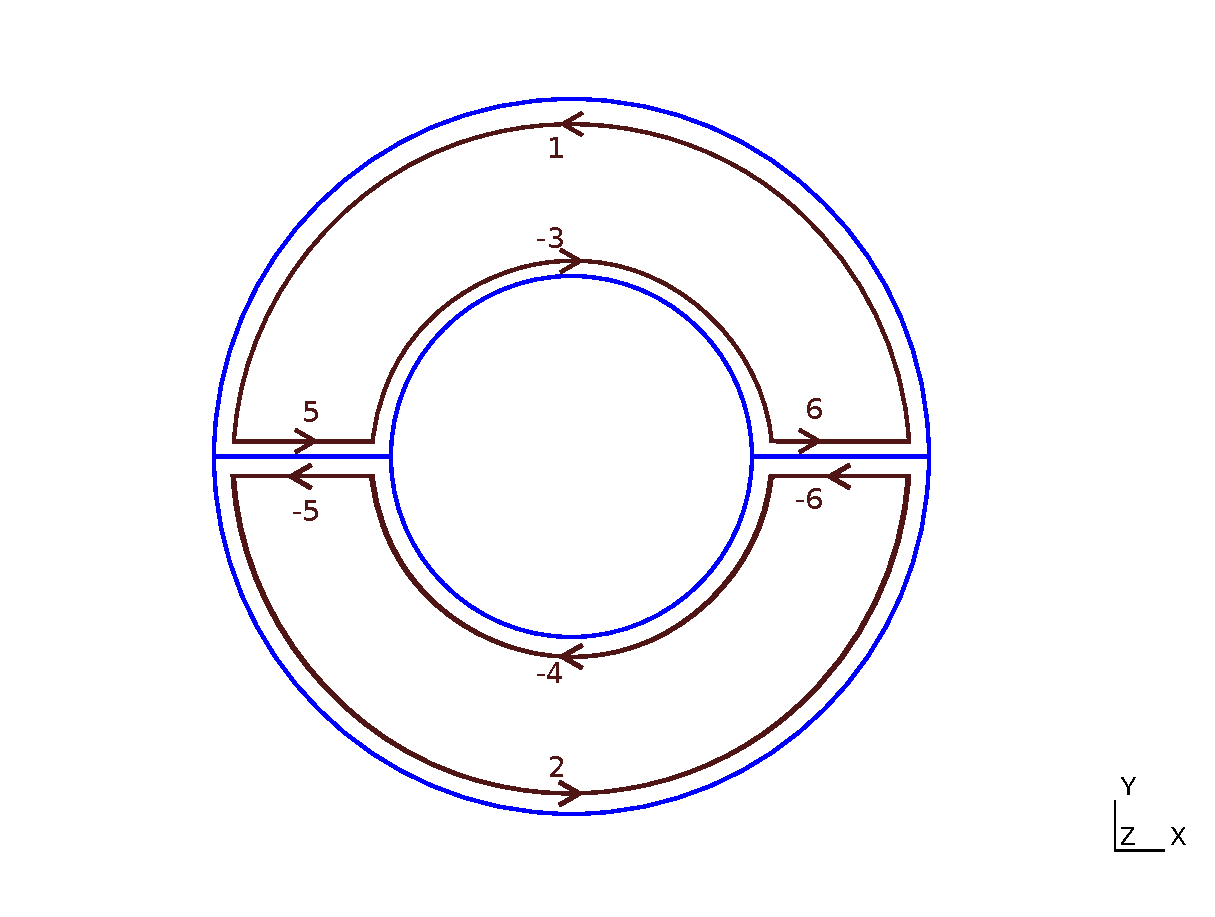
\includegraphics[width=12 cm]{anillo_contornos.pdf}
    \caption{Contornos de la geometría.}
    \label{fig:geo_contornos}
\end{figure}

Creamos, entonces, los contornos y luego las superficies correspondientes a cada contorno como
a continuación

\begin{minted}[mathescape,
numbersep=5pt,
gobble=0,
frame=lines,
framesep=2mm]{c}
// Bucles y superficies
Line Loop(7) = {1, 5, -3, 6};
Plane Surface(8) = {7};
Line Loop(9) = {2, -6, -4, -5};
Plane Surface(10) = {9};
\end{minted}

\subsubsection{Grupos físicos}
En Gmsh, los grupos físicos se refieren a conjuntos de entidades geométricas --puntos, líneas, superficies o volúmenes--. Estos conjuntos, o grupos, pueden usarse para denotar una región
de un dominio que posee las mismas características, por ejemplo: un mismo material, o
una condición de carga o empotramiento. En este caso vamos a definir dos líneas físicas, 
correspondientes con los radios interno y externo y una superficies física.

En el archivo de entrada sería
\begin{minted}[mathescape,
numbersep=5pt,
gobble=0,
frame=lines,
framesep=2mm]{c}
// Grupos fisicos
Physical Line(11) = {1, 2};
Physical Line(12) = {3, 4};
Physical Surface(13) = {8, 10};
\end{minted}


\subsection{Parámetros de malla en el archivo de entrada}
Adicionalmente, Gmsh permite definir ciertos parámetros que determinan la forma en la que se escribe
la malla. En este caso, queremos hacer una subdivisión de los arcos y líneas radiales, equivalente
a una rejilla en coordenadas cartesianas. Esto lo logramos especificando cuántas divisiones queremos
para las líneas que representan arcos y cuántas para las líneas radiales.

Eso se logra con

\begin{minted}[mathescape,
numbersep=5pt,
gobble=0,
frame=lines,
framesep=2mm]{c}
// Subdivision de lineas
ndiv_arco = 44;  // Subdivisiones de los arcos
ndiv_rad = 12;    // Subdivisiones en la direccion radial
Transfinite Line {5, 6} = ndiv_rad Using Progression 1;
Transfinite Line {1, 3, 4, 2} = ndiv_arco Using Progression 1;
\end{minted}

En el caso de la subdivisión de la superficie usamos

\begin{minted}[mathescape,
numbersep=5pt,
gobble=0,
frame=lines,
framesep=2mm]{c}
// Subdivision superficies
Transfinite Surface {8};
Transfinite Surface {10};
\end{minted}

Si, además, queremos que la malla use cuadriláteros en lugar de triángulos, podemos indicar en el
archivo de entrada que queremos unir los triángulo para formar cuadriláteros.

Esto se hace a usando

\begin{minted}[mathescape,
numbersep=5pt,
gobble=0,
frame=lines,
framesep=2mm]{c}
// Recombinar triangulos en cuadrilateros
Recombine Surface {8, 10};
\end{minted}


\subsection{Archivo de entrada completo}
El archivo \texttt{.geo} completo es el siguiente

\inputminted[mathescape,
numbersep=5pt,
gobble=0,
frame=lines,
framesep=2mm]{c}{img/discret/anillo.geo}

Para obtener la malla en la interfaz gráfica vamos a \texttt{Mesh/2D} o \texttt{Malla/2D}, si está en español. Desde una terminal podemos usar

\begin{minted}[mathescape,
numbersep=5pt,
gobble=0]{bash}
gmsh anillo.geo -2 -o anillo.msh
\end{minted}

En ambos casos, deberíamos obtener la malla deseada. Esta, debe lucir como la siguiente figura.
\begin{figure}[H]
    \centering
    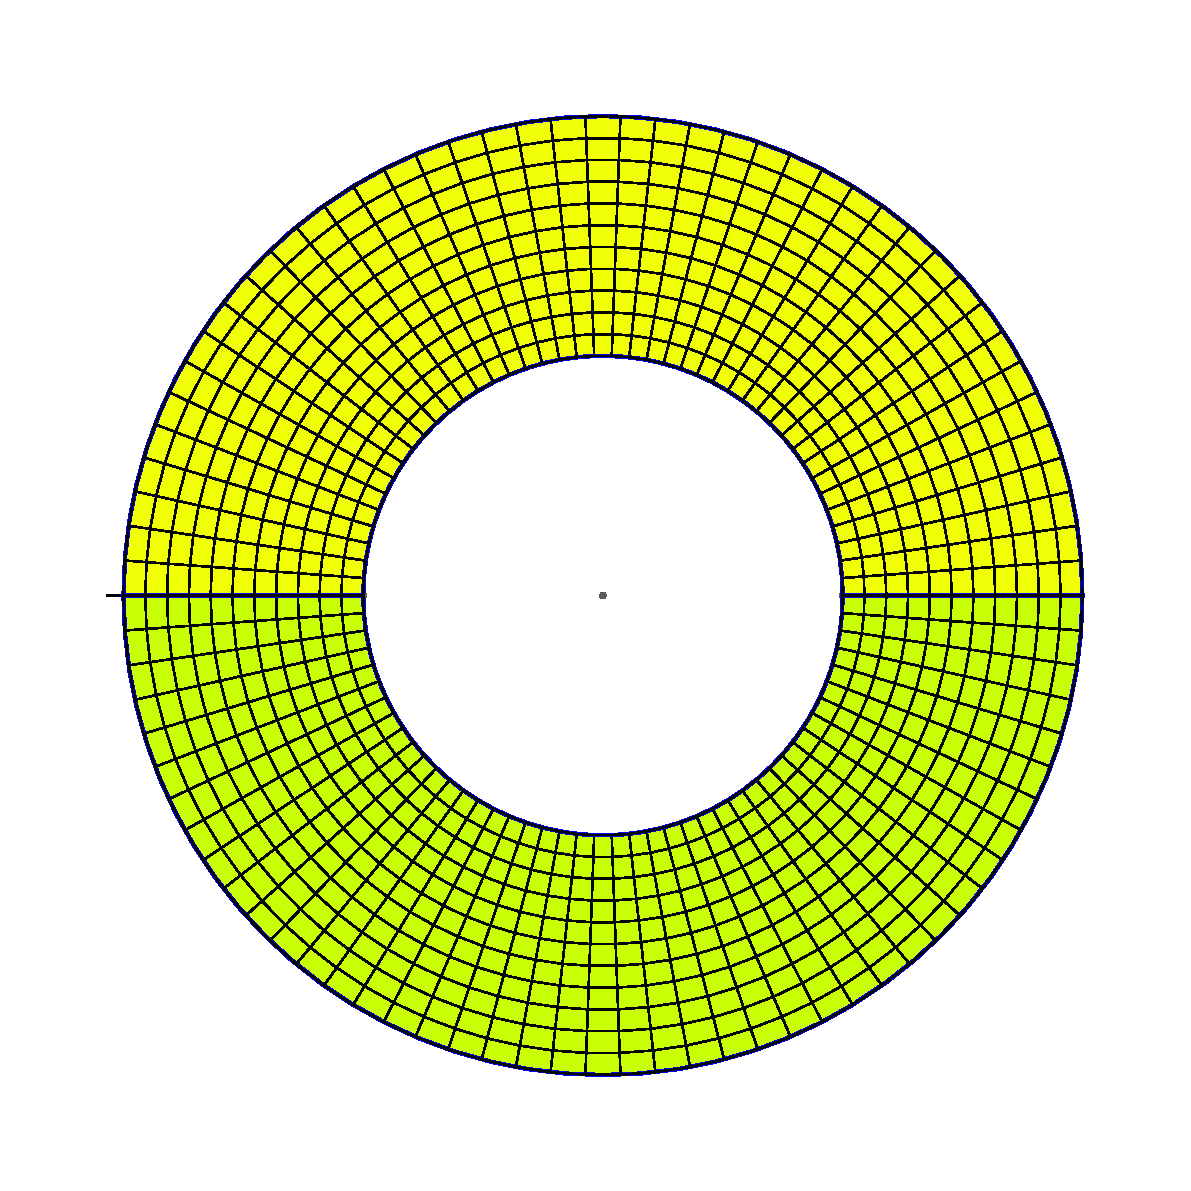
\includegraphics[width=10 cm]{anillo_msh.pdf}
    \caption{Malla para la geometría descrita.}
    \label{fig:malla}
\end{figure}


\section{Lectura de mallas de Gmsh desde Python}
Supongamos que tenemos un cuadrado de lado 1, dado por el siguiente archivo de Gmsh.
\inputminted[mathescape,
numbersep=5pt,
gobble=0,
frame=lines,
framesep=2mm]{c}{img/discret/cuadrado.geo}

Si mallamos este geometría en Gmsh, obtendríamos lo siguiente.
\begin{figure}[H]
    \centering
    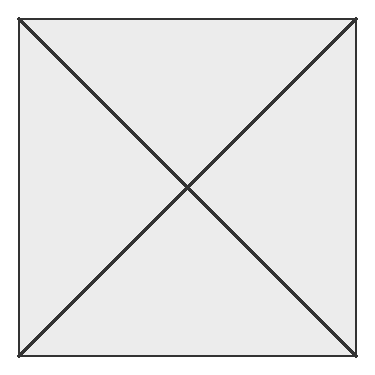
\includegraphics[width=2.5 in]{cuadrado_malla.pdf}
    \caption{Malla para la geometría descrita.}
    \label{fig:malla_cuadrado}
\end{figure}

El archivo (\texttt{.msh}) correspondiente a este malla es el siguiente.
\inputminted[mathescape,
numbersep=5pt,
gobble=0,
frame=lines,
linenos,
framesep=2mm]{bash}{img/discret/cuadrado.msh}

Podemos ver que los nodos están definidos entre la línea 5 y la línea 10. Y los 
elementos entre las líneas 14 y 25. Particularmente, los elementos 
triangulare\footnote{Los puntos y las líneas también se consideran elementos y 
por esto aparecen en el archivo, a menos que se especifique lo contrario.} 
están definidos entre las líneas 22 y 25. La primera columna en la sección de 
elementos (\texttt{\$Elements})\footnote{Esta información se encuentra en la 
documentación de Gmsh, disponible en: 
\url{http://gmsh.info/doc/texinfo/gmsh.html\#MSH-file-format-version-2}.} 
indica 
el número del elemento, las siguientes indican los grupos a los cuales 
pertenece, y a partir de la sexta columna tenemos la conectividad de los 
elementos.

Realizar un script de Python que lea este tipo de archivos no es una tarea difícil, sin embargo, sí es una tarea tediosa. El paquete \texttt{meshio}\footnote{Disponible en: \url{https://github.com/nschloe/meshio}.} nos permite leer estos archivos de forma simple.

El siguiente bloque de código leer este archivo.
\begin{minted}[mathescape,
numbersep=5pt,
gobble=0,
frame=lines,
framesep=2mm]{python}
import meshio

mesh = meshio.read("cuadrado.msh")
\end{minted}

Y luego podemos acceder a la información de la malla como se muestra en el siguiente bloque de código.
\begin{minted}[mathescape,
numbersep=5pt,
gobble=0,
frame=lines,
framesep=2mm]{python}
points = mesh.points
cells = mesh.cells
point_data = mesh.point_data
cell_data = mesh.cell_data
\end{minted}




